\documentclass{article}
%\documentstyle[11pt,handout,psfig]{article}

\usepackage{fullpage,amssymb,amsmath,epsf, color}
\usepackage[12pt]{extsizes}
\usepackage{algorithm}
\usepackage{algorithmic}

%These give really tight margins:
%\setlength{\topmargin}{-0.3in}
%\setlength{\textheight}{8.10in}
%\setlength{\textwidth}{5.8in}
%\setlength{\baselineskip}{0.1875in}
%\addtolength{\leftmargin}{-2.775in}123214444444444444444444444444444444444444444444444444444441
%\setlength{\footskip}{0.45in}
%\setlength{\oddsidemargin}{0.5in}
%\setlength{\evensidemargin}{0.5in}
%%\setlength{\headsep}{0pt}
%%\setlength{\headheight}{0pt}

%\setlength{\topmargin}{-0.5in}
\setlength{\textheight}{8in}
%\setlength{\textwidth}{5.0in}
%\setlength{\baselineskip}{0.1875in}
%\addtolength{\leftmargin}{-2.775in}
%\setlength{\footskip}{0.45in}
%\setlength{\oddsidemargin}{0.5in}
%\setlength{\evensidemargin}{0.5in}
%%\setlength{\headsep}{0pt}
%%\setlength{\headheight}{0pt}


\def\shownotes{1}  %set 1 to show author notes
\ifnum\shownotes=1
\newcommand{\authnote}[2]{$\ll$\textsf{\footnotesize #1 notes: #2}$\gg$}
\else
\newcommand{\authnote}[2]{}
\fi

\newcommand{\Tnote}[1]{{\color{blue}\authnote{Tengyu}{#1}}}

\markright{XCS229}
\pagestyle{myheadings}


\documentclass{article}
\usepackage[top = 1.0in]{geometry}

\usepackage{graphicx}

\usepackage[utf8]{inputenc}
\usepackage{listings}
\usepackage[dvipsnames]{xcolor}
\usepackage{bm}
\usepackage{algorithm}
\usepackage{algpseudocode}
\usepackage{framed}

\definecolor{codegreen}{rgb}{0,0.6,0}
\definecolor{codegray}{rgb}{0.5,0.5,0.5}
\definecolor{codepurple}{rgb}{0.58,0,0.82}
\definecolor{backcolour}{rgb}{0.95,0.95,0.92}

\lstdefinestyle{mystyle}{
    backgroundcolor=\color{backcolour},   
    commentstyle=\color{codegreen},
    keywordstyle=\color{magenta},
    stringstyle=\color{codepurple},
    basicstyle=\ttfamily\footnotesize,
    breakatwhitespace=false,         
    breaklines=true,                 
    captionpos=b,                    
    keepspaces=true,                 
    numbersep=5pt,                  
    showspaces=false,                
    showstringspaces=false,
    showtabs=false,                  
    tabsize=2
}

\lstset{style=mystyle}

\newcommand{\di}{{d}}
\newcommand{\nexp}{{n}}
\newcommand{\nf}{{p}}
\newcommand{\vcd}{{\textbf{D}}}
\newcommand{\Int}{\mathbb{Z}}
\newcommand\bb{\ensuremath{\mathbf{b}}}
\newcommand\bs{\ensuremath{\mathbf{s}}}
\newcommand\bp{\ensuremath{\mathbf{p}}}
\newcommand{\relu} { \operatorname{ReLU} }
\newcommand{\smx} { \operatorname{softmax} }
\newcommand\bx{\ensuremath{\mathbf{x}}}
\newcommand\bh{\ensuremath{\mathbf{h}}}
\newcommand\bc{\ensuremath{\mathbf{c}}}
\newcommand\bW{\ensuremath{\mathbf{W}}}
\newcommand\by{\ensuremath{\mathbf{y}}}
\newcommand\bo{\ensuremath{\mathbf{o}}}
\newcommand\be{\ensuremath{\mathbf{e}}}
\newcommand\ba{\ensuremath{\mathbf{a}}}
\newcommand\bu{\ensuremath{\mathbf{u}}}
\newcommand\bv{\ensuremath{\mathbf{v}}}
\newcommand\bP{\ensuremath{\mathbf{P}}}
\newcommand\bg{\ensuremath{\mathbf{g}}}
\newcommand\bX{\ensuremath{\mathbf{X}}}
% real numbers R symbol
\newcommand{\Real}{\mathbb{R}}

% encoder hidden
\newcommand{\henc}{\bh^{\text{enc}}}
\newcommand{\hencfw}[1]{\overrightarrow{\henc_{#1}}}
\newcommand{\hencbw}[1]{\overleftarrow{\henc_{#1}}}

% encoder cell
\newcommand{\cenc}{\bc^{\text{enc}}}
\newcommand{\cencfw}[1]{\overrightarrow{\cenc_{#1}}}
\newcommand{\cencbw}[1]{\overleftarrow{\cenc_{#1}}}

% decoder hidden
\newcommand{\hdec}{\bh^{\text{dec}}}

% decoder cell
\newcommand{\cdec}{\bc^{\text{dec}}}

\usepackage[hyperfootnotes=false]{hyperref}
\hypersetup{
  colorlinks=true,
  linkcolor = blue,
  urlcolor  = blue,
  citecolor = blue,
  anchorcolor = blue,
  pdfborderstyle={/S/U/W 1}
}
\usepackage{nccmath}
\usepackage{mathtools}
\usepackage{graphicx,caption}
\usepackage[shortlabels]{enumitem}
\usepackage{epstopdf,subcaption}
\usepackage{psfrag}
\usepackage{amsmath,amssymb,epsf}
\usepackage{verbatim}
\usepackage{cancel}
\usepackage{color,soul}
\usepackage{bbm}
\usepackage{listings}
\usepackage{setspace}
\usepackage{float}
\definecolor{Code}{rgb}{0,0,0}
\definecolor{Decorators}{rgb}{0.5,0.5,0.5}
\definecolor{Numbers}{rgb}{0.5,0,0}
\definecolor{MatchingBrackets}{rgb}{0.25,0.5,0.5}
\definecolor{Keywords}{rgb}{0,0,1}
\definecolor{self}{rgb}{0,0,0}
\definecolor{Strings}{rgb}{0,0.63,0}
\definecolor{Comments}{rgb}{0,0.63,1}
\definecolor{Backquotes}{rgb}{0,0,0}
\definecolor{Classname}{rgb}{0,0,0}
\definecolor{FunctionName}{rgb}{0,0,0}
\definecolor{Operators}{rgb}{0,0,0}
\definecolor{Background}{rgb}{0.98,0.98,0.98}
\lstdefinelanguage{Python}{
    numbers=left,
    numberstyle=\footnotesize,
    numbersep=1em,
    xleftmargin=1em,
    framextopmargin=2em,
    framexbottommargin=2em,
    showspaces=false,
    showtabs=false,
    showstringspaces=false,
    frame=l,
    tabsize=4,
    % Basic
    basicstyle=\ttfamily\footnotesize\setstretch{1},
    backgroundcolor=\color{Background},
    % Comments
    commentstyle=\color{Comments}\slshape,
    % Strings
    stringstyle=\color{Strings},
    morecomment=[s][\color{Strings}]{"""}{"""},
    morecomment=[s][\color{Strings}]{'''}{'''},
    % keywords
    morekeywords={import,from,class,def,for,while,if,is,in,elif,else,not,and,or
    ,print,break,continue,return,True,False,None,access,as,,del,except,exec
    ,finally,global,import,lambda,pass,print,raise,try,assert},
    keywordstyle={\color{Keywords}\bfseries},
    % additional keywords
    morekeywords={[2]@invariant},
    keywordstyle={[2]\color{Decorators}\slshape},
    emph={self},
    emphstyle={\color{self}\slshape},
%
}
\lstMakeShortInline|

\pagestyle{empty} \addtolength{\textwidth}{1.0in}
\addtolength{\textheight}{0.5in}
\addtolength{\oddsidemargin}{-0.5in}
\addtolength{\evensidemargin}{-0.5in}
\newcommand{\ruleskip}{\bigskip\hrule\bigskip}
\newcommand{\nodify}[1]{{\sc #1}}
\newenvironment{answer}{\sf \begingroup\color{ForestGreen}}{\endgroup}%

\setlist[itemize]{itemsep=2pt, topsep=0pt}
\setlist[enumerate]{itemsep=6pt, topsep=0pt}

\setlength{\parindent}{0pt}
\setlength{\parskip}{4pt}
\setlist[enumerate]{parsep=4pt}
\setlength{\unitlength}{1cm}

\renewcommand{\Re}{{\mathbb R}}
\newcommand{\R}{\mathbb{R}}
\newcommand{\what}[1]{\widehat{#1}}

\renewcommand{\comment}[1]{}
\newcommand{\mc}[1]{\mathcal{#1}}
\newcommand{\half}{\frac{1}{2}}

\DeclareMathOperator*{\argmin}{arg\,min}

\def\KL{D_{KL}}
\def\xsi{x^{(i)}}
\def\ysi{y^{(i)}}
\def\zsi{z^{(i)}}
\def\E{\mathbb{E}}
\def\calN{\mathcal{N}}
\def\calD{\mathcal{D}}
\def\slack{\url{http://xcs229-scpd.slack.com/}}
\def\zipscriptalt{\texttt{python zip\_submission.py}}
\DeclarePairedDelimiter\abs{\lvert}{\rvert}%
 
\usepackage{bbding}
\usepackage{pifont}
\usepackage{wasysym}
\usepackage{amssymb}
\usepackage{framed}
\usepackage{scrextend}

\newcommand{\alns}[1] {
	\begin{align*} #1 \end{align*}
}

\newcommand{\pd}[2] {
 \frac{\partial #1}{\partial #2}
}
\renewcommand{\Re} { \mathbb{R} }
\newcommand{\btx} { \mathbf{\tilde{x}} }
\newcommand{\bth} { \mathbf{\tilde{h}} }
\newcommand{\sigmoid} { \operatorname{\sigma} }
\newcommand{\CE} { \operatorname{CE} }
\newcommand{\byt} { \hat{\by} }
\newcommand{\yt} { \hat{y} }

\newcommand{\oft}[1]{^{(#1)}}
\newcommand{\fone}{\ensuremath{F_1}}

\newcommand{\ac}[1]{ {\color{red} \textbf{AC:} #1} }
\newcommand{\ner}[1]{\textbf{\color{blue} #1}}
\usepackage{graphicx}
\usepackage{subcaption}
%\renewcommand{\epsffile}[1]{
%	\includegraphics[width=\epsfxsize]{#1}
%}

\newcommand{\di}{{d}}
\newcommand{\nexp}{{n}}
\newcommand{\vcd}{{\textbf{D}}}




\begin{document}
\title{XCS229 Lecture Notes}
\author{Andrew Ng}
%\date{Updated by Tengyu Ma on \today}
\date{}
\maketitle



\setcounter{part}{8}
\part{The EM algorithm}

In the previous set of notes, we talked about the EM algorithm
as applied to fitting a mixture of Gaussians.  In this set of notes,
we give a broader view of the EM algorithm, and show how it can
be applied to a large family of estimation problems
with latent variables.  We begin our discussion with a very useful result
called {\bf Jensen's inequality}


\section{Jensen's inequality}

Let $f$ be a function whose domain is the set of real numbers.
Recall that $f$ is a convex function if $f''(x) \geq 0$ (for all $x \in \Re$).
In the case of $f$ taking vector-valued inputs, this is generalized to
the condition that its hessian $H$ is positive semi-definite ($H \geq 0$).
If $f''(x) > 0$ for all $x$, then we say $f$ is {\bf strictly} convex
(in the vector-valued case, the corresponding statement is that $H$ must
be positive definite, written $H > 0$).  Jensen's inequality
can then be stated as follows:

\medskip
\noindent
{\bf Theorem.} Let $f$ be a convex function, and let $X$ be a random variable.
Then:
\[
\E[f(X)] \geq f(\E X).
\]
Moreover, if $f$ is strictly convex, then
$\E[f(X)] = f(\E X)$ holds true if and only if $X = \E[X]$ with
probability 1 (i.e., if $X$ is a constant).
\medskip

Recall our convention of occasionally dropping the parentheses when
writing expectations, so in the theorem above, $f(\E X) = f(\E[X])$.

For an interpretation of the theorem, consider the figure below.

\begin{center}
% eps library outdated
% \epsfxsize=3in
% \epsffile{jensen.eps}
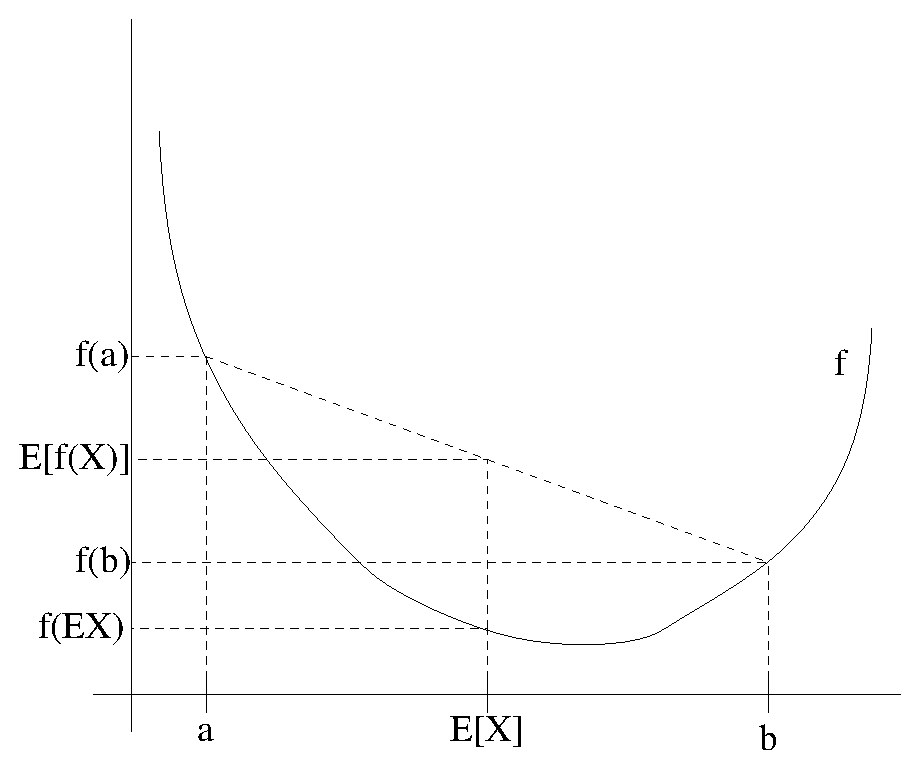
\includegraphics[scale=0.5]{jensen.eps}
\end{center}

Here, $f$ is a convex function shown by the solid line.  Also, $X$
is a random variable that has a 0.5 chance of taking the value $a$,
and a 0.5 chance of taking the value $b$ (indicated on the $x$-axis).
Thus, the expected value of $X$ is given by the midpoint
between $a$ and $b$.

We also see the values $f(a)$, $f(b)$ and $f(\E[X])$ indicated
on the $y$-axis.  Moreover, the value $\E[f(X)]$ is now
the midpoint on the $y$-axis between $f(a)$ and $f(b)$.  From
our example, we see that because $f$ is convex, it must be
the case that $\E[f(X)] \geq f(\E X)$.

Incidentally, quite a lot of people have trouble remembering which
way the inequality goes, and remembering a picture like this is
a good way to quickly figure out the answer.

\noindent
{\bf Remark.} Recall that $f$ is [strictly] concave if and only if $-f$ is
[strictly] convex (i.e., $f''(x) \leq 0$ or $H \leq 0$). Jensen's
inequality also holds for concave functions $f$, but with the direction
of all the inequalities reversed ($\E[f(X)] \leq f(\E X)$, etc.).



\section{The EM algorithm}

\newcommand{\cD}{\mathcal{D}}
Suppose we have an estimation problem in which
we have a training set $\{x^{(1)}, \ldots, x^{(\nexp)}\}$ consisting
of $\nexp$ independent examples.  We have a latent variable model $p(x,z;\theta)$ with $z$ being the latent variable (which for simplicity is assumed to take finite number of values). The density for $x$ can be obtained by marginalized over the latent variable $z$:
\begin{align}
p(x;\theta) = \sum_z p(x,z;\theta)
\end{align}


We wish to fit the parameters $\theta$ by maximizing the log-likelihood of the data, defined by
%wUltimately, we'd like to maximize the expected log-likelihood, denoted by $\bar{\ell}(\theta)$
%\begin{align}
%\bar{\ell}(\theta) = \E_{x\sim \cD}[\log p(x;\theta)]\label{eqn:expected}
%\end{align}
%where the expectation is taken over a test example $x$ drawn from the distribution $\cD$. Evaluating the expectation $\E_{x\sim \cD}$ exactly is not feasible because it requires infinite samples drawn from $\cD$, and therefore during the training, 
%We estimate the empirical log-likelihood defined by the training examples
\begin{eqnarray}
	\ell(\theta) &=& \sum_{i=1}^\nexp \log p(x^{(i)};\theta) \label{eqn:empirical}
%&=& \sum_{i=1}^\nexp \log \sum_z p(x,z; \theta).
\end{eqnarray}
We can rewrite the objective in terms of the joint density $p(x,z;\theta)$ by
\begin{eqnarray}
\ell(\theta) &=& \sum_{i=1}^\nexp \log p(x^{(i)};\theta) \\
&=& \sum_{i=1}^\nexp \log \sum_{z^{(i)}} p(x^{(i)},z^{(i)}; \theta).
\end{eqnarray}
But, explicitly finding the maximum likelihood estimates of the parameters
$\theta$ may be hard since it will result in difficult non-convex optimization problems.\footnote{It's mostly an empirical observation that the optimization problem is difficult to optimize.} Here, the $\zsi$'s are the latent random variables;
and it is often the case that if the $\zsi$'s were observed, then
maximum likelihood estimation would be easy.

In such a setting, the EM algorithm gives an efficient method for
maximum likelihood estimation.  Maximizing $\ell(\theta)$
explicitly might be difficult, and our strategy will be to instead
repeatedly
construct a lower-bound on $\ell$ (E-step), and then optimize
that lower-bound (M-step).\footnote{Empirically, the E-step and M-step can often be computed more efficiently than optimizing the function $\ell(\cdot)$ directly. However, it doesn't necessarily mean that alternating the two steps can always converge to the global optimum of $\ell(\cdot)$. Even for mixture of Gaussians, the EM algorithm can either converge to a global optimum or get stuck, depending on the properties of the training data. Empirically, for real-world data, often EM can converge to a solution with relatively high likelihood (if not the optimum), and the theory behind it is still largely not understood. }

%Note that $\ell(\theta)$ is an approximation of $\bar{\ell}(\theta)$ (by replacing the expectation by samples) up to a factor of $n$. At the end of the day, we will design an algorithm that optimize $\ell(\theta)$. However, it turns out it's mathematically cleaner to first think about how to optimize the expected log-likelihood $\bar{\theta}$ (so that we don't have to deal with the superscript.) Therefore, our plan is to introduce an algorithm for optimizing~\eqref{eqn:expected} first, and finally 
%of a model $p(x,z)$ to the data, 
It turns out that the summation $\sum_{i=1}^\nexp$ is not essential here, and towards a simpler exposition of the EM algorithm, we will first consider optimizing the the likelihood $\log p(x)$ for {\bf a single example $x$}. After we derive the algorithm for optimizing $\log p(x)$, we will convert it to an algorithm that works for $\nexp$ examples by adding back the sum to each of the relevant equations. Thus, now we aim to optimize $\log p(x;\theta)$ which can be rewritten as
\begin{align}
\log p(x;\theta) = \log \sum_z p(x,z; \theta)
\end{align}
Let $Q$ be a distribution over the possible values of $z$.  That is, $\sum_z Q(z) = 1$, $Q(z) \geq 0$). 

Consider the following:\footnote{If $z$ were continuous, then $Q$
	would be a density, and the summations over $z$ in our discussion
	are replaced with integrals over $z$.}
\begin{eqnarray}
\log p(x; \theta)
&=&  \log \sum_{z} p(x, z; \theta) \nonumber\\
&=& \log \sum_{z} Q(z) \frac{p(x, z; \theta)}{Q(z)} \label{eqn-em1-z}\\
&\geq&  \sum_{z} Q(z) \log \frac{p(x, z; \theta)}{Q(z)} \label{eqn-em2-z}
\end{eqnarray}



%HERE: Error... log x is concave.  Need to fix, and check how well it ties
%in with the rest of the notes, since I think I used convexity mostly.
The last step of this derivation used Jensen's inequality.  Specifically,
$f(x) = \log x$ is a concave function, since $f''(x) = -1/x^2 < 0$ over its
domain $x \in \Re^+$.  Also, the term
\[
\sum_{z} Q(z) \left[\frac{p(x, z; \theta)}{Q(z)}\right]
\]
in the summation is just an expectation of the quantity
$\left[p(x, z; \theta)/Q(z)\right]$ with respect to $z$
drawn according to the distribution given by $Q$.\footnote{We note that the notion $\frac{p(x, z; \theta)}{Q(z)}$ only makes sense if $Q(z) \neq 0$ whenever $p(x,z;\theta)\neq 0$. Here we implicitly assume that we only consider those $Q$ with such a property.}
By Jensen's inequality, we have
\[
f\left(\E_{z \sim Q}
\left[
\frac{p(x, z; \theta)}{Q(z)}\right] \right)
\geq
\E_{z \sim Q}
\left[
f\left(
\frac{p(x, z; \theta)}{Q(z)}\right) \right],
\]
where the ``$z \sim Q$'' subscripts above indicate that the expectations
are with respect to $z$ drawn from $Q$.
This allowed us to go from Equation~(\ref{eqn-em1-z}) to
Equation~(\ref{eqn-em2-z}).
%By Jensen's
%inequality, $f(\E X) \leq \E[f(X)]$, which implied Equation~(\ref{eqn-em2}).

Now, for {\bf any} distribution $Q$, the formula~(\ref{eqn-em2-z})
gives a lower-bound on $\log p(x;\theta)$.
There are many possible choices for the $Q$'s.  Which should we choose?
Well, if we have some current guess $\theta$ of the parameters, it seems
natural to try to make the lower-bound tight at that value of $\theta$.
I.e., we will make the inequality above hold with equality at our
particular value of $\theta$. 

% (We'll see later how this enables us
%to prove that $\ell(\theta)$ increases monotonically with successive
%iterations of EM.)

To make the bound tight for a particular value of $\theta$, we need
for the step involving Jensen's inequality in
our derivation above to hold with equality. For this to be true,
we know it is sufficient that the expectation
be taken over a ``constant''-valued random variable.  I.e., we require
that
\[
\frac{p(x, z; \theta)}{Q(z)} = c
\]
for some constant $c$ that does not depend on $z$. This is
easily accomplished by choosing
\[
Q(z) \propto p(x, z; \theta).
\]
Actually, since we know $\sum_z Q(z) = 1$ (because it is a distribution),
this further tells us that
\begin{eqnarray}
	Q(z) &=& \frac{p(x, z; \theta)}{\sum_z p(x, z; \theta)} \nonumber\\
	&=& \frac{p(x, z; \theta)}{p(x; \theta)} \nonumber\\
	&=& p(z | x; \theta)\label{eqn:Q}
\end{eqnarray}
Thus, we simply set the $Q$'s to be the posterior distribution of
the $z$'s given $x$ and the setting of the parameters $\theta$.


Indeed, we can directly verify that when $Q(z) = p(z | x; \theta)$, then equation~\eqref{eqn-em2-z} is an equality because 
\begin{align}
%Q(z) = p(z | x; \theta) & \textup{~~implies} \\
\sum_{z} Q(z) \log \frac{p(x, z; \theta)}{Q(z)} & = \sum_{z} p(z | x;\theta) \log \frac{p(x, z; \theta)}{p(z | x;\theta)} \nonumber\\
&= \sum_{z} p(z | x;\theta) \log \frac{p(z | x; \theta) p(x;\theta)}{p(z | x;\theta)} \nonumber\\
& = \sum_{z} p(z | x;\theta) \log p(x;\theta) \nonumber\\
& = \log p(x;\theta) \sum_{z} p(z | x; \theta) \nonumber \\
& = \log p(x; \theta) \tag{because $\sum_{z} p(z | x;\theta)=1$}
\end{align}

\newcommand{\elbo}{\textup{ELBO}}

For convenience, we call the expression in Equation~\eqref{eqn-em2-z} the {\bf evidence lower bound} (ELBO) and we denote it by
\begin{align}
\elbo(x; Q, \theta) = \sum_{z} Q(z) \log \frac{p(x, z; \theta)}{Q(z)}  \label{eqn:elbo-z}
\end{align}
With this equation, we can re-write equation~\eqref{eqn-em2-z} as
\begin{align}
\forall Q, \theta, x,~~~ \log p(x;\theta) \ge \elbo(x;Q,\theta) \label{eqn-em3}
\end{align}
Intuitively, the EM algorithm alternatively updates $Q$ and $\theta$ by a) setting $Q(z) = p(z | x; \theta)$ following Equation~\eqref{eqn:Q} so that $\elbo(x;Q,\theta) = \log p(x;\theta)$ for $x$ and the current $\theta$, and b) maximizing $\elbo(x;Q,\theta)$ w.r.t $\theta$ while fixing the choice of $Q$. 

Recall that all the discussion above was under the assumption that we aim to optimize the log-likelihood $\log p(x;\theta)$ for a single example $x$. It turns out that with multiple training examples, the basic idea is the same and we only needs to take a sum over examples at relevant places. Next, we will build the evidence lower bound for multiple training examples and make the EM algorithm formal. 

Recall we have a training set $\{x^{(1)}, \ldots, x^{(\nexp)}\}$. Note that the optimal choice of $Q$ is $p(z | x;\theta)$, and it depends on the particular example $x$. Therefore here we will introduce $\nexp$ distributions $Q_1,\dots, Q_{\nexp}$, one for each example $x^{(i)}$. For each example $x^{(i)}$, we can build the evidence lower bound 
\begin{align}
\log p(\xsi;\theta) \ge \elbo(\xsi; Q_i,\theta) = \sum_{\zsi} Q_i(\zsi) \log \frac{p(\xsi, \zsi; \theta)}{Q_i(\zsi)}\nonumber
\end{align}
Taking sum over all the examples, we obtain a lower bound for the log-likelihood 
\begin{align}
\ell(\theta) &\ge \sum_i \elbo(\xsi; Q_i,\theta) \label{eqn-em2} \\
& = \sum_i \sum_{\zsi} Q_i(\zsi) \log \frac{p(\xsi, \zsi; \theta)}{Q_i(\zsi)}\nonumber
\end{align}

%Now, for this choice of the $Q$'s, Equation~(\ref{eqn-em2}) gives
%a lower-bound on the loglikelihood $\ell$ that we're trying to maximize.
%This is the E-step.  In the M-step of the algorithm, we then maximize
%our formula in Equation~(\ref{eqn-em2}) with respect to
%the parameters to obtain a new setting of the $\theta$'s.  Repeatedly
%carrying out these two steps gives us the EM algorithm, which is as follows:
%\begin{itemize}
%	\item[] Repeat until convergence $\{$
%	\begin{itemize}
%		\item[] (E-step) For each $i$, set
%		\[
%		Q(z) := p(z | x; \theta).
%		\]
%		\item[] (M-step) Set
%		\[
%		\theta := \arg \max_\theta \sum_i \sum_z Q(z) \log \frac{p(x,z;\theta)}{Q(z)}.
%		\]
%	\end{itemize}
%	\item[] $\}$
%\end{itemize}
%
%How do we know if this algorithm will converge?  Well, suppose
%$\theta^{(t)}$ and $\theta^{(t+1)}$ are the parameters from two
%successive iterations of EM.  We will now prove that
%$\ell(\theta^{(t)}) \leq \ell(\theta^{(t+1)})$, which shows
%EM always monotonically improves the log-likelihood.
%The key to showing this result lies in our choice of the $Q$'s.
%Specifically, on the iteration of EM in which the parameters
%had started out as $\theta^{(t)}$, we would have chosen
%$Q^{(t)}(z) := p(z | x; \theta^{(t)})$.  We saw
%earlier that this choice ensures that Jensen's inequality,
%as applied to get Equation~(\ref{eqn-em2}), holds with equality,
%and hence
%\[
%\ell(\theta^{(t)}) =
%\sum_i \sum_z Q^{(t)}(z) \log \frac{p(x,z;\theta^{(t)})}{Q^{(t)}(z)}.
%\]
%The parameters $\theta^{(t+1)}$ are then obtained by maximizing
%the right hand side of the equation above.  Thus,
%\begin{eqnarray}
%\ell(\theta^{(t+1)}) &\geq&
%\sum_i \sum_z Q^{(t)}(z) \log \frac{p(x,z;\theta^{(t+1)})}{Q^{(t)}(z)}\\
%&\geq&
%\sum_i \sum_z Q^{(t)}(z) \log \frac{p(x,z;\theta^{(t)})}{Q^{(t)}(z)}
%\label{eqn-emproof2} \\
%&=& \ell(\theta^{(t)})
%\label{eqn-emproof3}
%\end{eqnarray}
%This first inequality comes from the fact that
%\[
%\ell(\theta) \geq
%\sum_i \sum_z Q(z) \log \frac{p(x,z;\theta)}{Q(z)}
%\]
%holds for any values of $Q$ and $\theta$, and in particular holds for
%$Q = Q^{(t)}$, $\theta=\theta^{(t+1)}$.
%To get Equation~(\ref{eqn-emproof2}), we used the fact that
%$\theta^{(t+1)}$ is chosen explicitly to be
%\[
%\arg\max_\theta \sum_i \sum_z Q(z) \log \frac{p(x,z;\theta)}{Q(z)},
%\]
%and thus this formula evaluated at $\theta^{(t+1)}$ must be equal to or larger
%than the same formula evaluated at $\theta^{(t)}$.  Finally, the step
%used to get~(\ref{eqn-emproof3}) was shown earlier, and follows from
%$Q^{(t)}$ having been chosen to make Jensen's inequality hold with
%equality at $\theta^{(t)}$.
%
%Hence, EM causes the likelihood to converge monotonically.  In our description
%of the EM algorithm, we said we'd run it until convergence. Given the result
%that we just showed, one reasonable convergence test would be to check if
%the increase in
%$\ell(\theta)$ between successive iterations is smaller than some
%tolerance parameter, and to declare convergence if EM is improving
%$\ell(\theta)$ too slowly.
%









%where the likelihood is given by
%\begin{eqnarray*}
%\ell(\theta) &=& \sum_{i=1}^\nexp \log p(x;\theta) \\
%&=& \sum_{i=1}^\nexp \log \sum_z p(x,z; \theta).
%\end{eqnarray*}

%Generally maximizing $\log p(x;\theta)$ (or the corresponding multiple sample version in~\eqref{eqn:empirical}) using the formula above  and it is often the case that if the $z$ is observed, then maximum likelihood estimation would be easy. 
%maximum likelihood estimation would be easy.

%But, explicitly finding the maximum likelihood estimates of the parameters
%$\theta$ may be hard.  Here, the $\zsi$'s are the latent random variables;
%and it is often the case that if the $\zsi$'s were observed, then
%maximum likelihood estimation would be easy.

%In such a setting, the EM algorithm gives an efficient method for
%maximum likelihood estimation.  Maximizing $\ell(\theta)$
%explicitly might be difficult, and our strategy will be to instead
%repeatedly
%construct a lower-bound on $\ell$ (E-step), and then optimize
%that lower-bound (M-step).

%For each $i$, let $Q_i$ be some distribution
%over the $z$'s ($\sum_z Q_i(z) = 1$, $Q_i(z) \geq 0$).
%Consider the following:\footnote{If $z$ were continuous, then $Q_i$
%would be a density, and the summations over $z$ in our discussion
%are replaced with integrals over $z$.}
%\begin{eqnarray}
%\sum_i \log p(\xsi; \theta)
%&=& \sum_i \log \sum_{\zsi} p(\xsi, \zsi; \theta) \\
%&=& \sum_i \log \sum_{\zsi} Q_i(\zsi) \frac{p(\xsi, \zsi; \theta)}{Q_i(\zsi)} \label{eqn-em1}\\
%&\geq& \sum_i \sum_{\zsi} Q_i(\zsi) \log \frac{p(\xsi, \zsi; \theta)}{Q_i(\zsi)} \label{eqn-em2}
%\end{eqnarray}
%%HERE: Error... log x is concave.  Need to fix, and check how well it ties
%%in with the rest of the notes, since I think I used convexity mostly.
%The last step of this derivation used Jensen's inequality.  Specifically,
%$f(x) = \log x$ is a concave function, since $f''(x) = -1/x^2 < 0$ over its
%domain $x \in \Re^+$.  Also, the term
%\[
%\sum_{\zsi} Q_i(\zsi) \left[\frac{p(\xsi, \zsi; \theta)}{Q_i(\zsi)}\right]
%\]
%in the summation is just an expectation of the quantity
%$\left[p(\xsi, \zsi; \theta)/Q_i(\zsi)\right]$ with respect to $\zsi$
%drawn according to the distribution given by $Q_i$.
%By Jensen's inequality, we have
%\[
%f\left(\E_{\zsi \sim Q_i}
%\left[
%\frac{p(\xsi, \zsi; \theta)}{Q_i(\zsi)}\right] \right)
%\geq
%\E_{\zsi \sim Q_i}
%\left[
%f\left(
%\frac{p(\xsi, \zsi; \theta)}{Q_i(\zsi)}\right) \right],
%\]
%where the ``$\zsi \sim Q_i$'' subscripts above indicate that the expectations
%are with respect to $\zsi$ drawn from $Q_i$.
%This allowed us to go from Equation~(\ref{eqn-em1}) to
%Equation~(\ref{eqn-em2}).
%%By Jensen's
%%inequality, $f(\E X) \leq \E[f(X)]$, which implied Equation~(\ref{eqn-em2}).

For \emph{any} set of distributions $Q_1,\dots ,Q_{\nexp}$, the formula~(\ref{eqn-em2})
gives a lower-bound on $\ell(\theta)$, and analogous to the argument around equation~\eqref{eqn:Q}, the $Q_i$ that attains equality satisfies
%There're many possible choices for the $Q_i$'s.  Which should we choose?
%Well, if we have some current guess $\theta$ of the parameters, it seems
%natural to try to make the lower-bound tight at that value of $\theta$.
%I.e., we'll make the inequality above hold with equality at our
%particular value of $\theta$.  (We'll see later how this enables us
%to prove that $\ell(\theta)$ increases monotonically with successive
%iterations of EM.)
%To make the bound tight for a particular value of $\theta$, we need
%for the step involving Jensen's inequality in
%our derivation above to hold with equality. For this to be true,
%we know it is sufficient that the expectation
%be taken over a ``constant''-valued random variable.  I.e., we require
%that
%\[
%\frac{p(\xsi, \zsi; \theta)}{Q_i(\zsi)} = c
%\]
%for some constant $c$ that does not depend on $\zsi$. This is
%easily accomplished by choosing
%\[
%Q_i(\zsi) \propto p(\xsi, \zsi; \theta).
%\]
%Actually, since we know $\sum_z Q_i(\zsi) = 1$ (because it is a distribution),
%this further tells us that
\begin{eqnarray*}
Q_i(\zsi)% &=& \frac{p(\xsi, \zsi; \theta)}{\sum_z p(\xsi, z; \theta)} \\
%&=& \frac{p(\xsi, \zsi; \theta)}{p(\xsi; \theta)} \\
&=& p(\zsi | \xsi; \theta)
\end{eqnarray*}
Thus, we simply set the $Q_i$'s to be the posterior distribution of
the $\zsi$'s given $\xsi$ with the current setting of the parameters $\theta$.

Now, for this choice of the $Q_i$'s, Equation~(\ref{eqn-em2}) gives
a lower-bound on the loglikelihood $\ell$ that we're trying to maximize.
This is the E-step.  In the M-step of the algorithm, we then maximize
our formula in Equation~(\ref{eqn-em2}) with respect to
the parameters to obtain a new setting of the $\theta$'s.  Repeatedly
carrying out these two steps gives us the EM algorithm, which is as follows:
\begin{itemize}
\item[] Repeat until convergence $\{$
\begin{itemize}
\item[] (E-step) For each $i$, set
\[
Q_i(\zsi) := p(\zsi | \xsi; \theta).
\]
\item[] (M-step) Set
\begin{align}
\theta &:= \arg \max_\theta \sum_{i=1}^\nexp \elbo(\xsi; Q_i,\theta) \nonumber\\
& = \arg \max_\theta \sum_i \sum_\zsi Q_i(\zsi) \log \frac{p(\xsi,\zsi;\theta)}{Q_i(\zsi)}.
\end{align}
\end{itemize}
\item[] $\}$
\end{itemize}

How do we know if this algorithm will converge?  Well, suppose
$\theta^{(t)}$ and $\theta^{(t+1)}$ are the parameters from two
successive iterations of EM.  We will now prove that
$\ell(\theta^{(t)}) \leq \ell(\theta^{(t+1)})$, which shows
EM always monotonically improves the log-likelihood.
The key to showing this result lies in our choice of the $Q_i$'s.
Specifically, on the iteration of EM in which the parameters
had started out as $\theta^{(t)}$, we would have chosen
$Q_i^{(t)}(\zsi) := p(\zsi | \xsi; \theta^{(t)})$.  We saw
earlier that this choice ensures that Jensen's inequality,
as applied to get Equation~(\ref{eqn-em2}), holds with equality,
and hence
\begin{align}
\ell(\theta^{(t)}) = \sum_{i=1}^\nexp \elbo(\xsi; Q^{(t)}_i,\theta^{(t)}) \label{eqn:QQ}
%\sum_i \sum_\zsi Q_i^{(t)}(\zsi) \log \frac{p(\xsi,\zsi;\theta^{(t)})}{Q_i^{(t)}(\zsi)}.
\end{align}
The parameters $\theta^{(t+1)}$ are then obtained by maximizing
the right hand side of the equation above.  Thus,
\begin{align}
\ell(\theta^{(t+1)}) &\geq
\sum_{i=1}^\nexp \elbo(\xsi; Q^{(t)}_i,\theta^{(t+1)}) \tag{because ineqaulity~\eqref{eqn-em2} holds for all $Q$ and $\theta$} \\
&\geq
\sum_{i=1}^\nexp \elbo(\xsi; Q^{(t)}_i,\theta^{(t)}) \tag{see reason below}\\
& = \ell(\theta^{(t)}) \tag{by equation~\eqref{eqn:QQ}}
\label{eqn-emproof3}
\end{align}
where the last inequality follows from that $\theta^{(t+1)}$ is chosen explicitly to be
\[
\arg\max_\theta  ~~\sum_{i=1}^\nexp\elbo(\xsi; Q^{(t)}_i,\theta) %= \arg\max_\theta  \sum_i \sum_\zsi Q_i(\zsi) \log \frac{p(\xsi,\zsi;\theta)}{Q_i(\zsi)},
\]
%This first inequality comes from the fact that
%\[
%\ell(\theta) \geq
%\sum_i \sum_\zsi Q_i(\zsi) \log \frac{p(\xsi,\zsi;\theta)}{Q_i(\zsi)}
%\]
%holds for any values of $Q_i$ and $\theta$, and in particular holds for
%$Q_i = Q_i^{(t)}$, $\theta=\theta^{(t+1)}$.
%To get Equation~(\ref{eqn-emproof2}), we used the fact that
%$\theta^{(t+1)}$ is chosen explicitly to be
%\[
%\arg\max_\theta  \elbo(\xsi; Q^{(t)}_i,\theta) %= \arg\max_\theta  \sum_i \sum_\zsi Q_i(\zsi) \log \frac{p(\xsi,\zsi;\theta)}{Q_i(\zsi)},
%\]
%and thus this formula evaluated at $\theta^{(t+1)}$ must be equal to or larger
%than the same formula evaluated at $\theta^{(t)}$.  Finally, the step
%used to get~(\ref{eqn-emproof3}) was shown earlier, and follows from
%$Q_i^{(t)}$ having been chosen to make Jensen's inequality hold with
%equality at $\theta^{(t)}$.

Hence, EM causes the likelihood to converge monotonically.  In our description
of the EM algorithm, we said we'd run it until convergence. Given the result
that we just showed, one reasonable convergence test would be to check if
the increase in
$\ell(\theta)$ between successive iterations is smaller than some
tolerance parameter, and to declare convergence if EM is improving
$\ell(\theta)$ too slowly.

\bigskip
\noindent
{\bf Remark.} If we define (by overloading $\elbo(\cdot)$)
\begin{align}
\elbo(Q, \theta) = \sum_{i=1}^\nexp \elbo(\xsi; Q_i,\theta) = \sum_i \sum_\zsi Q_i(\zsi) \log \frac{p(\xsi, \zsi; \theta)}{Q_i(\zsi)} \label{eqn:elbo}
\end{align}
then we know $\ell(\theta) \geq \elbo(Q, \theta)$ from our previous derivation.
The EM can also be viewed an alternating maximization algorithm on $\elbo(Q, \theta) $, in which the E-step
maximizes it with respect to $Q$ (check this yourself), and the M-step
maximizes it with respect to $\theta$. %For certain cases, $\elbo(Q,\theta)$ is convex in variable $Q$ when $\theta$ is treated as fixed, or vice versa, but not convex jointly in variable $(Q,\theta)$. However, 
%This gives another view of why
%EM must converge monotonically.
%\medskip
\newcommand{\kl}{D_{KL}}
\subsection{Other interpretation of ELBO}

Let $\elbo(x;Q,\theta)= \sum_{z} Q(z) \log \frac{p(x, z; \theta)}{Q(z)}$ be defined as in equation~\eqref{eqn:elbo-z}. There are several other forms of ELBO. First, we can rewrite 
\begin{align}
\elbo(x;Q,\theta) & = \E_{z \sim Q}[\log p(x,z;\theta)] -  \E_{z \sim Q}[\log Q(z)]  \nonumber\\
& =  \E_{z\sim Q}[\log p(x | z; \theta)] - \kl(Q\| p_z)\label{eqn:1}
\end{align}
where we use $p_z$ to denote the marginal distribution of $z$ (under the distribution $p(x,z;\theta)$), and $\kl()$ denotes the KL divergence 
\begin{align}
\kl(Q\| p_z) = \sum_z Q(z)\log \frac{Q(z)}{p(z)}
\end{align}
In many cases, the marginal distribution of $z$ does not depend on the parameter $\theta$. In this case, we can see that maximizing $\elbo$ over $\theta$ is equivalent to maximizing the first term in~\eqref{eqn:1}. This corresponds to maximizing the conditional likelihood of $x$ conditioned on $z$, which is often a simpler question than the original question.  

Another form of $\elbo(\cdot)$ is (please verify yourself)
\begin{align}
\elbo(x; Q,\theta) = \log p(x) - \kl(Q\|p_{z|x})
\end{align}
where $p_{z|x}$ is the conditional distribution of $z$ given $x$ under the parameter $\theta$. This forms shows that the maximizer of $\elbo(Q,\theta)$ over $Q$ is obtained when $Q = p_{z|x}$, which was shown in equation~\eqref{eqn:Q} before. 
\section{Mixture of Gaussians revisited}\label{sec:gmm}

Armed with our general definition of the EM algorithm, let's go back
to our old
example of fitting the parameters $\phi$, $\mu$ and $\Sigma$ in
a mixture of Gaussians.  For the sake of brevity, we carry out
the derivations for the M-step updates only for $\phi$ and $\mu_j$,
and leave the updates for $\Sigma_j$ as an exercise for the reader.

The E-step is easy.  Following our algorithm derivation above,
we simply calculate
\[
w^{(i)}_j = Q_i(z^{(i)}=j) = P(\zsi=j | \xsi; \phi, \mu, \Sigma).
\]
Here, ``$Q_i(z^{(i)}=j)$'' denotes the probability of $\zsi$ taking the
value $j$
under the distribution $Q_i$.

Next, in the M-step, we need to maximize, with respect to our parameters
$\phi, \mu, \Sigma$, the quantity
\begin{eqnarray*}
&&\hbox to -0.3in{}\sum_{i=1}^\nexp \sum_{\zsi} Q_i(\zsi)
   \log \frac{p(\xsi, \zsi; \phi, \mu, \Sigma)}{Q_i(\zsi)}  \\
&&= \sum_{i=1}^\nexp \sum_{j=1}^k Q_i(\zsi=j) \log \frac{p(\xsi| \zsi = j; \mu, \Sigma) p(\zsi=j; \phi)}{Q_i(\zsi=j)}  \\
&&=
\sum_{i=1}^\nexp \sum_{j=1}^k w^{(i)}_j \log \frac{\frac{1}{(2\pi)^{\di/2}|\Sigma_j|^{1/2}}
\exp\left(-\frac{1}{2}(\xsi-\mu_j)^T\Sigma_j^{-1}(\xsi-\mu_j)\right) \cdot \phi_j}
{w^{(i)}_j}
\end{eqnarray*}
Let's maximize this with respect to $\mu_l$.  If we take the
derivative with respect to $\mu_l$, we find
\begin{eqnarray*}
&&\hbox to -0.5in{}
\nabla_{\mu_l} \sum_{i=1}^\nexp \sum_{j=1}^k w^{(i)}_j \log \frac{\frac{1}{(2\pi)^{\di/2}|\Sigma_j|^{1/2}}
\exp\left(-\frac{1}{2}(\xsi-\mu_j)^T\Sigma_j^{-1}(\xsi-\mu_j)\right) \cdot \phi_j}
{w^{(i)}_j} \\
\hbox to 0.2in{}&=&
- \nabla_{\mu_l} \sum_{i=1}^\nexp \sum_{j=1}^k w^{(i)}_j
\frac{1}{2}(\xsi-\mu_j)^T\Sigma_j^{-1}(\xsi-\mu_j) \\
&=&
\frac{1}{2} \sum_{i=1}^\nexp w^{(i)}_l \nabla_{\mu_l}
2 \mu_l^T \Sigma_l^{-1} \xsi - \mu_l^T\Sigma_l^{-1}\mu_l \\
&=&
\sum_{i=1}^\nexp w^{(i)}_l
\left( \Sigma_l^{-1}\xsi - \Sigma_l^{-1}\mu_l \right)
\end{eqnarray*}
Setting this to zero and solving for $\mu_l$ therefore yields the
update rule
\[
\mu_l := \frac{\sum_{i=1}^\nexp w^{(i)}_l    \xsi}{\sum_{i=1}^\nexp w^{(i)}_l    }, \\
\]
which was what we had in the previous set of notes.

Let's do one more example, and derive the M-step update
for the parameters $\phi_j$.  Grouping together only the terms that depend
on $\phi_j$, we find that we need to maximize
\[
\sum_{i=1}^\nexp \sum_{j=1}^k w^{(i)}_j \log \phi_j.
\]
However, there is an additional constraint that the $\phi_j$'s sum to 1,
since they represent the probabilities $\phi_j = p(\zsi=j ;\phi)$.
To deal with the constraint that $\sum_{j=1}^k \phi_j =1$, we construct
the Lagrangian
\[
\calL(\phi) = \sum_{i=1}^\nexp \sum_{j=1}^k w^{(i)}_j \log \phi_j + \beta (\sum_{j=1}^k \phi_j -1),
\]
where $\beta$ is the Lagrange multiplier.\footnote{We don't need to worry about
the constraint that $\phi_j \geq 0$, because as we'll shortly see, the
solution we'll find from this derivation will automatically satisfy
that anyway.}
Taking derivatives, we find
\[
\frac{\partial}{\partial \phi_j} \calL(\phi) = \sum_{i=1}^\nexp \frac{w^{(i)}_j}{\phi_j} + \beta
\]
Setting this to zero and solving, we get
\[
\phi_j = \frac{\sum_{i=1}^\nexp w_j^{(i)}}{-\beta}
\]
I.e., $\phi_j \propto \sum_{i=1}^\nexp w_j^{(i)}$.  Using the constraint that
$\sum_j \phi_j = 1$, we easily find that
$-\beta = \sum_{i=1}^\nexp \sum_{j=1}^k w_j^{(i)} = \sum_{i=1}^\nexp 1 = \nexp$.
(This used the fact that $w_j^{(i)} = Q_i(\zsi=j)$, and
since probabilities sum to 1, $\sum_j w_j^{(i)}=1$.) We therefore have
our M-step updates for the parameters $\phi_j$:
\[
\phi_j := \frac{1}{\nexp} \sum_{i=1}^\nexp w^{(i)}_j.
\]

The derivation for the M-step updates to $\Sigma_j$ are also entirely
straightforward.

\section{Variational inference and variational auto-encoder}

\newcommand{\cN}{\mathcal{N}}
Loosely speaking, variational auto-encoder~\cite{kingma2013auto} generally refers to a family of algorithms that extend the EM algorithms to more complex models parameterized by neural networks. It extends the technique of variational inference with the additional ``re-parametrization trick'' which will be introduced below. Variational auto-encoder may not give the best performance for many datasets, but it contains several central ideas about how to extend EM algorithms to high-dimensional continuous latent variables with non-linear models. Understanding it will likely give you the language and backgrounds to understand various recent papers related to it.  

As a running example, we will consider the following parameterization of $p(x,z;\theta)$ by a neural network. Let $\theta$ be the collection of the weights of a neural network $g(z;\theta)$ that maps $z\in \mathbb{R}^k$ to $\mathbb{R}^{\di}$. Let 
\begin{align}
z & \sim \cN(0, I_{k\times k}) \\
x\vert z & \sim \cN(g(z;\theta),\sigma^2 I_{\di \times \di}) \label{eqn:mlp}
\end{align}
Here $I_{k\times k}$ denotes identity matrix of dimension $k$ by $k$, and $\sigma$ is a scalar that we assume to be known for simplicity. 



For the Gaussian mixture models in Section~\ref{sec:gmm}, the optimal choice of $Q(z)=p(z | x; \theta)$ for each fixed $\theta$, that is the posterior distribution of $z$, can be analytically computed. In many more complex models such as the model~\eqref{eqn:mlp}, it's intractable to compute the exact the posterior distribution $p(z | x;\theta)$. 

Recall that from equation~\eqref{eqn-em3}, ELBO is always a lower bound for any choice of $Q$, and therefore, we can also aim for finding an {\bf approximation} of the true posterior distribution. Often, one has to use some particular form to approximate the true posterior distribution. Let $\mathcal{Q}$ be a family of $Q$'s that we are considering, and we will aim to find a $Q$ within the family of $\mathcal{Q}$ that is closest to the true posterior distribution. To formalize, recall the definition of the ELBO lower bound as a function of $Q$ and $\theta$ defined in equation~\eqref{eqn:elbo}
\begin{align}
\elbo(Q, \theta) = \sum_{i=1}^\nexp \elbo(\xsi; Q_i,\theta) = \sum_i \sum_\zsi Q_i(\zsi) \log \frac{p(\xsi, \zsi; \theta)}{Q_i(\zsi)} \nonumber
\end{align}

Recall that EM can be viewed as alternating maximization of $\elbo(Q,\theta)$. Here instead, we optimize the EBLO over $Q\in \mathcal{Q}$
\begin{align}
\max_{Q\in \mathcal{Q}}\max_{\theta} \elbo(Q, \theta) \label{eqn:meta}
\end{align}

Now the next question is what form of $Q$ (or what structural assumptions to make about $Q$) allows us to efficiently maximize the objective above. When the latent variable $z$ are high-dimensional discrete variables, one popular assumption is the {\bf mean field assumption}, which assumes that $Q_i(z)$ gives a distribution with independent coordinates, or in other words, $Q_i$ can be decomposed into $Q_i(z) = Q_i^1(z_1)\cdots Q_i^k(z_k)$. There are tremendous applications of mean field assumptions to learning generative models with discrete latent variables, and we refer to~\cite{blei2017variational} for a survey of these models and their impact to a wide range of applications including computational biology, computational neuroscience, social sciences.  We will not get into the details about the discrete latent variable cases, and our main focus is to deal with continuous latent variables, which requires not only mean field assumptions, but additional techniques. 

When $z\in \mathbb{R}^k$ is a continuous latent variable, there are several decisions to make towards successfully optimizing~\eqref{eqn:meta}. First we need to give a succinct representation of the distribution $Q_i$ because it is over an infinite number of points. A natural choice is to assume $Q_i$ is a Gaussian distribution with some mean and variance. We would also like to have more succinct representation of the means of $Q_i$ of all the examples. %If the means of $Q_i$'s are independent parameters, the number of parameters will scale in $\nexp$, which potentially will cause overfitting. 
Note that $Q_i(\zsi)$ is supposed to approximate $p(z^{(i)} | x^{(i)}; \theta)$. It would make sense let all the means of the $Q_i$'s be some function of $x^{(i)}$. Concretely, let $q(\cdot;\phi), v(\cdot; \phi)$ be two functions that map from dimension $\di$ to $k$, which are parameterized by $\phi$ and $\psi$, we assume that 
\begin{align}
Q_i = \cN(q(\xsi;\phi), \textup{diag}(v(\xsi;\psi))^2)\label{eqn:Qigaussian}
\end{align}

Here $\textup{diag}(w)$ means the $k\times k$ matrix with the entries of $w\in \mathbb{R}^k$ on the diagonal. In other words, the distribution $Q_i$ is assumed to be a Gaussian distribution with independent coordinates, and the mean and standard deviations are governed by $q$ and $v$. Often in variational auto-encoder, $q$ and $v$ are chosen to be neural networks.\footnote{$q$ and $v$ can also share parameters.  We sweep this level of details under the rug in this note.} In recent deep learning literature, often $q, v$ are called {\bf encoder} (in the sense of encoding the data into latent code), whereas $g(z;\theta)$ if often referred to as the {\bf decoder.}

%Typically $v(\xsi,\psi)\in \mathbb{R}^{k\times k}$ is assumed to be a diagonal matrix which simplifies the implementation a lot. Although our discussion of the methodology here is oblivious to such simplification. 

We remark that $Q_i$ of such form in many cases are very far from a good approximation of the true posterior distribution. However, some approximation is necessary for feasible optimization. In fact, the form of $Q_i$ needs to satisfy other requirements (which happened to be satisfied by the form~\eqref{eqn:Qigaussian}) 

Before optimizing the ELBO, let's first verify whether we can efficiently evaluate the value of the ELBO for fixed $Q$ of the form~\eqref{eqn:Qigaussian} and $\theta$. We rewrite the ELBO as a function of $\phi, \psi, \theta$ by 
\begin{align}
\elbo(\phi,\psi,\theta) & = \sum_{i=1}^{\nexp}\E_{\zsi \sim Q_i}\left[\log \frac{p(\xsi,\zsi;\theta)}{Q_i(\zsi)}\right], \\
& \textup{ where } Q_i = \cN(q(\xsi;\phi), \textup{diag}(v(\xsi;\psi))^2) \nonumber
\end{align}
Note that to evaluate $Q_i(\zsi)$ inside the expectation, we should be able {\bf to compute the density of $Q_i$}. 
To estimate the expectation $\E_{\zsi \sim Q_i}$, we should be able {\bf to sample from distribution $Q_i$} so that we can build an empirical estimator with samples.  It happens that for Gaussian distribution $ Q_i = \cN(q(\xsi;\phi), \textup{diag}(v(\xsi;\psi))^2)$, we are able to be both efficiently. 

Now let's optimize the ELBO. It turns out that we can run gradient ascent over $\phi, \psi, \theta$ instead of alternating maximization. There is no strong need to compute the maximum over each variable at a much greater cost. (For Gaussian mixture model in Section~\ref{sec:gmm}, computing the maximum is analytically feasible and relatively cheap, and therefore we did alternating maximization.) Mathematically, let $\eta$ be the learning rate, the gradient ascent step is 
\begin{align}
\theta & : = \theta + \eta \nabla_\theta \elbo(\phi,\psi,\theta)\nonumber \\
\phi & : = \phi + \eta \nabla_\phi \elbo(\phi,\psi,\theta) \nonumber\\
\psi & : = \psi + \eta \nabla_\psi \elbo(\phi,\psi,\theta) \nonumber
\end{align}
Computing the gradient over $\theta$ is simple because 
\begin{align}
 \nabla_\theta \elbo(\phi,\psi,\theta) &=  \nabla_\theta \sum_{i=1}^{\nexp}\E_{\zsi \sim Q_i}\left[\frac{\log p(\xsi,\zsi;\theta)}{Q_i(\zsi)}\right] \nonumber \\
&=  \nabla_\theta \sum_{i=1}^{\nexp}\E_{\zsi \sim Q_i}\left[ \log p(\xsi,\zsi;\theta)\right] \nonumber \\
&= \sum_{i=1}^{\nexp}\E_{\zsi \sim Q_i}\left[\nabla_\theta \log p(\xsi,\zsi;\theta)\right],
\end{align}

But computing the gradient over $\phi$ and $\psi$ is tricky because the sampling distribution $Q_i$ depends on $\phi$ and $\psi$. (Abstractly speaking, the issue we face can be simplified as the problem of computing the gradient $\E_{z\sim Q_\phi}[f(\phi)]$ with respect to variable $\phi$. We know that in general, $\nabla \E_{z\sim Q_\phi}[f(\phi)] \neq \E_{z\sim Q_\phi}[\nabla f(\phi)]$ because the dependency of $Q_\phi$ on $\phi$ has to be taken into account as well. )

The idea that comes to rescue is the so-called {\bf re-parameterization trick}: we rewrite $\zsi \sim Q_i = \cN(q(\xsi;\phi), \textup{diag}(v(\xsi;\psi))^2)$ in an equivalent way: 
\begin{align}
\zsi = q(\xsi;\phi) + v(\xsi;\psi)  \odot \xi^{(i)} \textup{ where }\xi^{(i)}\sim \cN(0,I_{k\times k})
\end{align}

Here $x \odot y$ denotes the entry-wise product of two vectors of the same dimension. Here we used the fact that $x\sim N(\mu, \sigma^2)$ is equivalent to that $x = \mu + \xi \sigma$ with $\xi\sim N(0,1)$. We mostly just used this fact in every dimension simultaneously for the random variable $z^{(i)} \sim Q_i$. 

With this re-parameterization, we have that 
\begin{align}
& \E_{\zsi \sim Q_i}\left[\log \frac{p(\xsi,\zsi;\theta)}{Q_i(\zsi)}\right] \\
& = \E_{\xi^{(i)}\sim \cN(0,1)}\left[\log \frac{p(\xsi,q(\xsi;\phi) + v(\xsi;\psi)\odot \xi^{(i)};\theta)}{Q_i(q(\xsi;\phi) + v(\xsi;\psi)\odot \xi^{(i)} )}\right]\nonumber
\end{align}

It follows that 
\begin{align}
& \nabla_\phi \E_{\zsi \sim Q_i}\left[\log \frac{p(\xsi,\zsi;\theta)}{Q_i(\zsi)}\right] \nonumber\\
& =  \nabla_\phi \E_{\xi^{(i)}\sim \cN(0,1)}\left[\log \frac{p(\xsi,q(\xsi;\phi) + v(\xsi;\psi)\odot \xi^{(i)};\theta)}{Q_i(q(\xsi;\phi) + v(\xsi;\psi)\odot \xi^{(i)} )}\right]\nonumber\\
& =  \E_{\xi^{(i)}\sim \cN(0,1)}\left[ \nabla_\phi\log \frac{p(\xsi,q(\xsi;\phi) + v(\xsi;\psi)\odot \xi^{(i)};\theta)}{Q_i(q(\xsi;\phi) + v(\xsi;\psi)\odot \xi^{(i)} )}\right]\nonumber
\end{align}

We can now sample multiple copies of $\xi^{(i)}$'s to estimate the the expectation in the RHS of the equation above.\footnote{Empirically people sometimes just use one sample to estimate it for maximum computational efficiency.} We can estimate the gradient with respect to $\psi$ similarly, and with these, we can implement the gradient ascent algorithm to optimize the ELBO over $\phi, \psi, \theta.$

There are not many high-dimensional distributions with analytically computable density function are known to be re-parameterizable. We refer to ~\cite{kingma2013auto} for a few other choices that can replace Gaussian distribution. 
% Then, we can have the following variational inference meta-algorithm. (We call it a meta-algorithm to emphasize the fact that there might be various ways to instantiate the algorithms with all the details.)
%
%
%\begin{itemize}
%	\item[] Repeat until convergence $\{$
%	\begin{itemize}
%		\item[] (E-step) For each example $i$, find $Q_i(z^{(i)})$ such that 
%		\[
%		Q_i(\zsi) \approx p(\zsi | \xsi; \theta).
%		\]
%		\item[] (M-step) Set
%		\[
%		\theta := \arg \max_\theta \sum_{i=1}^\nexp \elbo(\xsi; Q_i,\theta) = \arg \max_\theta \sum_{i=1}^{\nexp}\E_{\zsi \sim Q_i}\left[\log \frac{p(\xsi,\zsi;\theta)}{Q_i(\zsi)}\right].
%		\]
%	\end{itemize}
%	\item[] $\}$
%\end{itemize}

%Alternatively, the M-step can be replaced by one gradient ascent step over the variable $\theta$ since computing the exact maximum may be too expensive. 
%\begin{align}
%\theta := \theta + \eta \nabla \sum_{i=1}^\nexp \elbo(\xsi; Q_i,\theta) = \theta + \eta \nabla \E_{\zsi \sim Q_i}\left[\log \frac{p(\xsi,\zsi;\theta)}{Q_i(\zsi)}\right].
%\end{align}

%When $z$ is in a continuous space, we also need a parametric form for the distribution $Q$. Suppose we parameterize $Q$ by $\phi$ and therefore the density of $z$ is given by $Q(z;\phi)$.

%\begin{center}
%\epsfxsize=3in
%\epsffile{foo.eps}
%\end{center}
\bibliography{cs229-notes8}
\bibliographystyle{plain}
\end{document}


